\chapter{Experimentos y Resultados}
\hrule \bigskip \vspace*{1cm}
%------------------------------------------------------------------------

En este trabajo, se considero  los datos de uso en el pecho como WESAD-Chest y los datos de uso en la muñeca como WESAD-Wrist.


\begin{figure}[h]
    \centering
    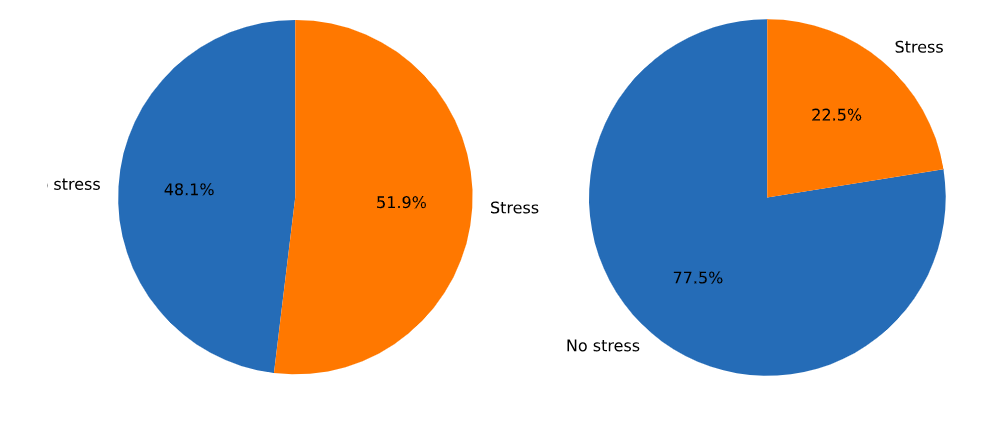
\includegraphics[width=7cm]{Graficos/stress.png}
    %\caption{Caption}
    \label{fig:enter-label}
\end{figure}



\begin{figure}[h]
    \centering
    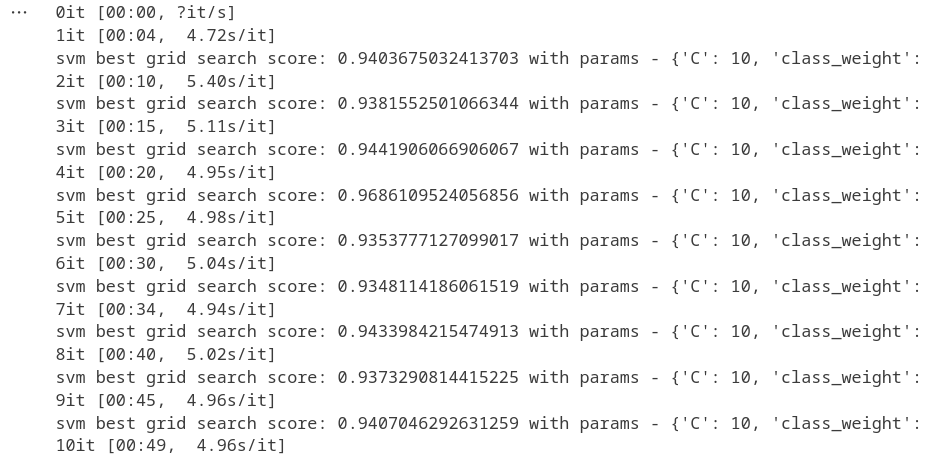
\includegraphics[width=7cm]{Graficos/capturaresutado.png}
    \caption{resultados}
    \label{fig:enter-label}
\end{figure}


\subsection{Métricas}

 La mayoría de estos conjuntos de datos tienen un  números desigual de etiquetas de estrés/no estrés,por lo que usar la precisión como se uso en otros trabajos no es adecuado,para evitar sesgos  se elige una métrica de evaluación basada en el estudio  de   Sirko Straube et al. [ Sirko Straube et al, 2020], donde establece que la precisión equilibrada (BA)  es una opción adecuada para evaluar los resultados,ya que se quiere evaluar la capacidad de   distinguir las dos categorías para evaluar solamente  la precisión de detectar patrones de estrés.


 

%----- Figura dos columnas.
\begin{figure*}[!tb] 
 \centering

 \caption{Ejemplo del \emph{aliasing} que se produce en una grilla con $N = 8$ nodos. Ambos modos
          ($k = 2$ y $k = 10$) toman los mismos valores en los puntos de la grilla.} \label{fig-2}
\end{figure*}
%----- Fin. Figura dos columnas.
